\documentclass[lualatex,aspectratio=169]{beamer}

\usepackage[utf8]{inputenc}
\usepackage[T1]{fontenc}
\usepackage{xspace}

\title{Accelerating $k$-D Trees for Nearest Neighbor Search on Walk-on-Spheres}
\date[\today]{\today}
\author[Ryan Smith]{Ryan Smith}


\newcommand{\kd}{$k$-D\xspace}

\usetheme{NIST}

\begin{document}

\begin{frame}
  \titlepage
\end{frame}

\begin{frame} 

  \frametitle{Outline} 
  %\framesubtitle{The proof uses \textit{reductio ad absurdum}.} 

  \begin{itemize} 
    \item Motivation and specification
    \item Introduction to \kd trees
    \item Limitations of \kd trees
    \item Flattened \kd trees
    \item Implementation details
    \item Performance results
    \item Areas for improvement
  \end{itemize}

\end{frame}



\begin{frame}
  \frametitle{Motivation}
  \framesubtitle{ZENO/Walk-on-Spheres}

  \begin{figure}
    \centering
    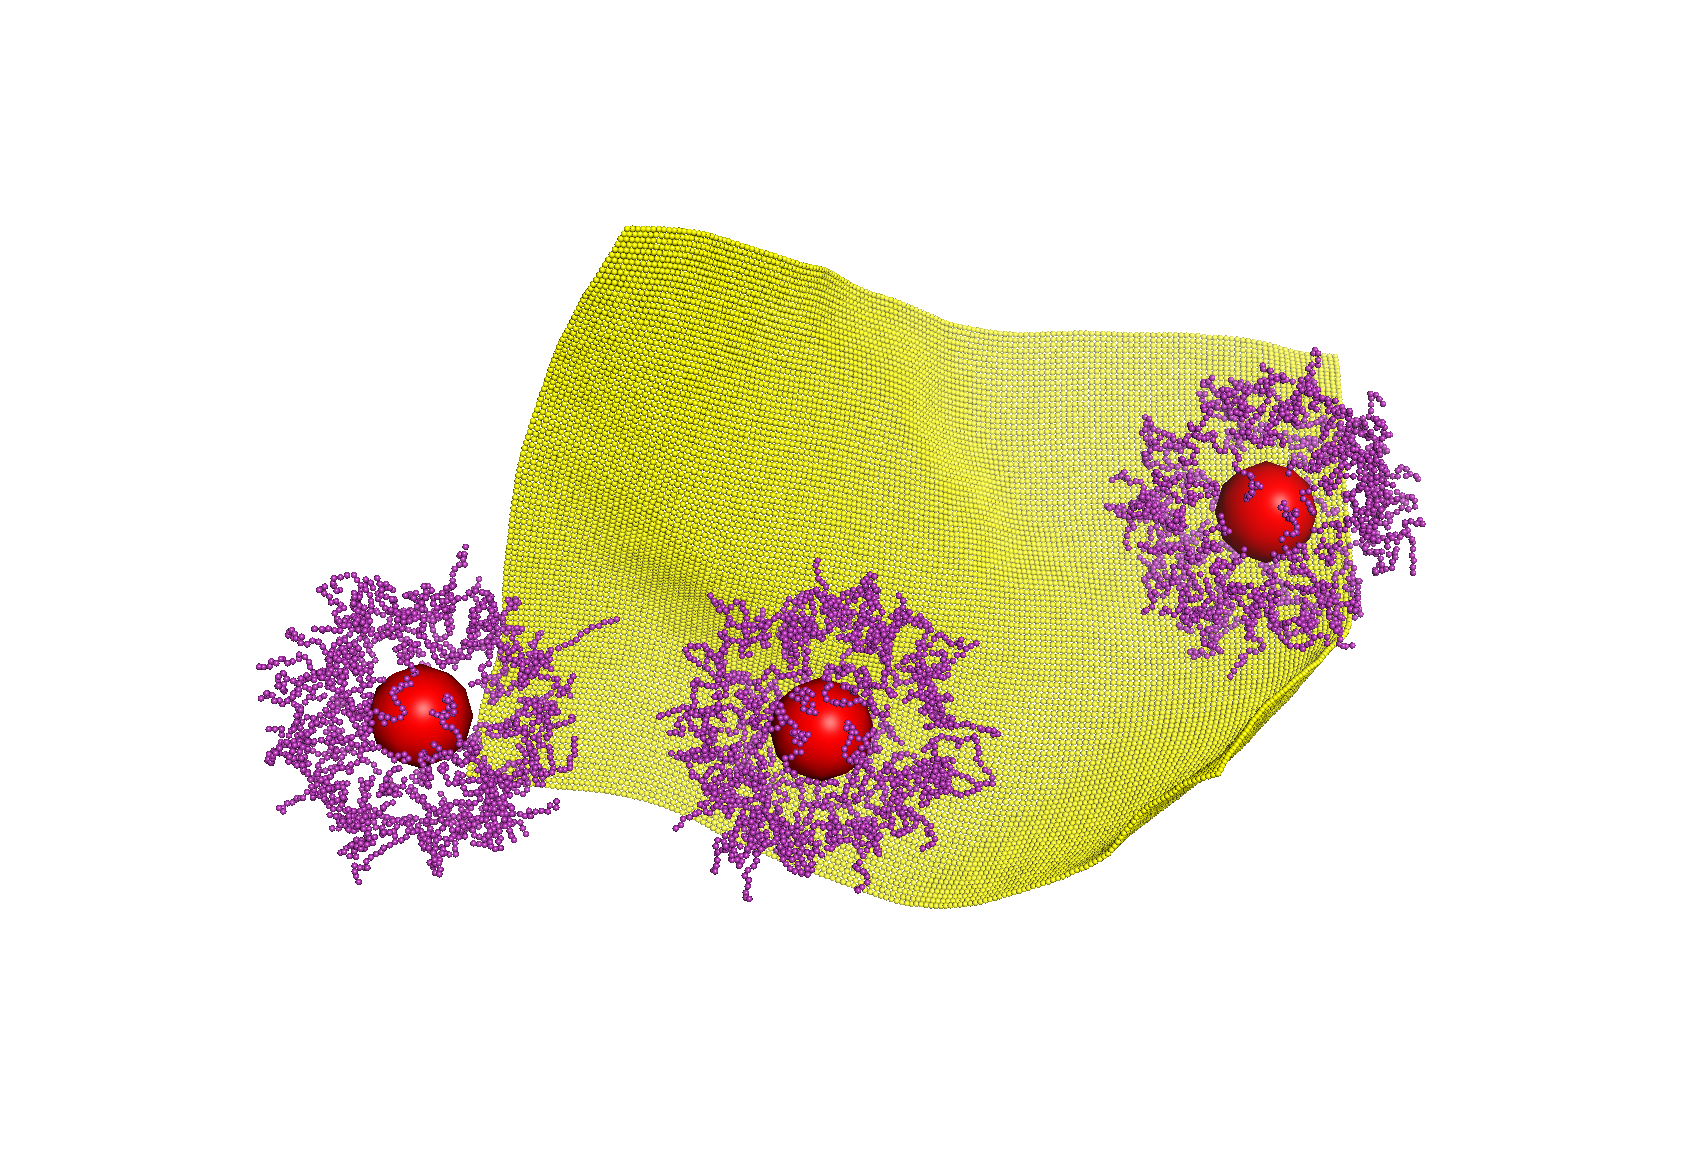
\includegraphics[width=0.7\textwidth]{80000.png}
    \caption{alkjasjj;}
    \label{fig:80000}
  \end{figure}

\end{frame}

\begin{frame}
  \frametitle{Motivation}
  \framesubtitle{ZENO/Walk-on-Spheres}

  \begin{itemize}
    \item Walk-on-Spheres accelerates Brownian Motion by jumping to a uniformly distributed point on the surface
      of a surrounding sphere
    \item The radius of the surrounding sphere is the distance of the random walker to the closest point in
      the molecule
    \item Our implementation uses \kd trees to quickly find the nearest neighbor
    \item The random access pattern of a \kd tree limits its potential for use on GPUs where memory operations
      are highly costly
  \end{itemize}

\end{frame}

\begin{frame}
  \frametitle{Specification}

  Improve performance of nearest neighbor search on \kd trees by more compactly organizing tree components
  to reduce cache misses and load instructions.

\end{frame}


\end{document}
